\documentclass[10pt, a4paper]{article}
\usepackage[utf8]{inputenc}
\usepackage{listings}
\usepackage{pgfplotstable}
\pgfplotsset{
	compat=1.13,
}
\usepgfplotslibrary{colormaps}

\title{Heuristic Analysis}
\author{Nathan Findley}
\date{March 2017}

\begin{document}

\maketitle
\tableofcontents

\begin{abstract}
	Evaluation of different search algorithms in a planning problem involving movement of cargo
	between airports via plane.
\end{abstract}

\section{Optimal Plan}

The order of presidence when evaluating an optimal plan is perhaps debatable
but I would consider time to find the path be the most essential constraint followed
perhaps by the length of the path in the evaluation of a real world problem.  Take for
instance the actual planning of shipments, the time taken to plan routes is quite critical
when it comes to customer satisfaction, but the actual plan itself could, if unnecessarily long,
result in extreme costs of shipping.

Fortunately given the data presented below, there really isn't much debate to be had about the
best plan of action: Breadth First Search is a winner.  Greedy Best First Graph Search H1 is a
tempting choice if the time elapsed for calculation of the plan is extremely important, but given that it produces
a route that is nearly twice as long a Breadth First Search it is doubtful that it would actually
be useful in a shipping context.

\section{Comparisons}

Breadth First Search and Depth First Search have significant differences in results: DFS is extremely quick when it comes to finding a solution.  Unfortunately
the path that was found was generally an order of magnitude larger than the path found by BFS, leaving DFS as an unlikely candidate in the real world.

Breadth First Search and Uniform Cost Search appear to be about on par with one another.  They are similar algothrithms so this shouldn't come as a surprise.
On all counts BFS is anywhere from moderately to significantly better than UCS.  While their path lengths are the same, time elapsed makes BFS a clear winner.

\section{A* Heuristics}
- Compare and contrast heuristic search result metrics using A* with the "ignore preconditions" and "level-sum" heuristics for Problems 1, 2, and 3.
- What was the best heuristic used in these problems?  Was it better than non-heuristic search planning methods for all problems?  Why or why not?

A* results contrast significantly depending on whether or not the heuristic involved is "ignore preconditions" or "level-sum".  The ignore preconditions heuristic
is roughly on par with BFS though it does appear to take more time.  Level-Sum, on the other hand, is much more time consuming.

I did not find, unfortunately, that A* was the best approach.  Breadth First Search appears to be a much better algorithm for this type of First Order Logic
path finding problem.  When I say best, I am indicating that the balance of path found and time elapsed are favorable.  
I do have to wonder if my implementation might possibly be incorrect since, according to my understanding, A* is considered to be the 
best search algorithm available.  If, however, you ignore the time taken, then, quite suddenly, A* using the level-sum heuristic beats everything else available
based on the given metrics.
I can say this because, while I have not included it specifically in this report, 
problem 3 will run at about 12.5 minutes for A* (level-sum) and it will find the 12 step path which means
that all other metrics are significantly lower than all other algorithms.

\section{Charts}

Zero value data points indicate that a 10 minute timeout was reached.

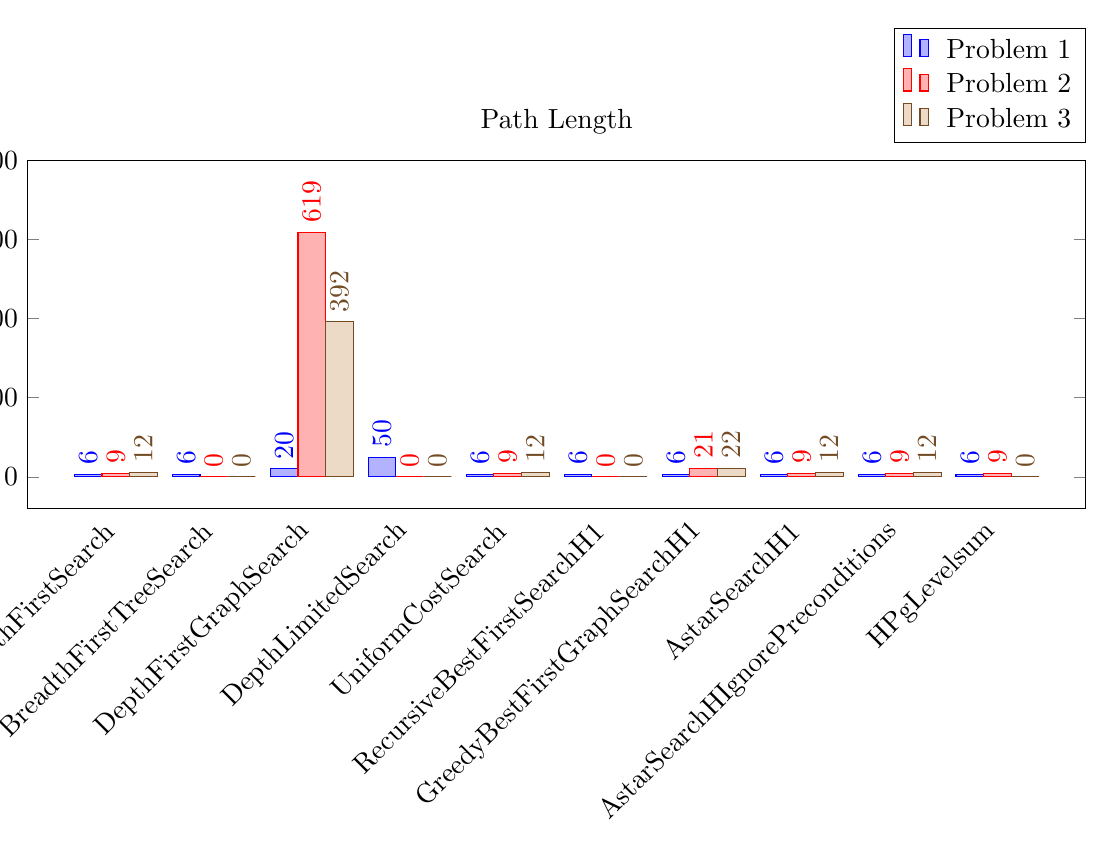
\begin{tikzpicture}[trim axis left, trim axis right]
	\begin{axis}[
			title={Path Length},
			major x tick style = transparent,
			ybar=0pt,
			ymax=800,
			symbolic x coords={
				BreadthFirstSearch,
				BreadthFirstTreeSearch,
				DepthFirstGraphSearch,
				DepthLimitedSearch,
				UniformCostSearch,
				RecursiveBestFirstSearchH1,
				GreedyBestFirstGraphSearchH1,
				AstarSearchH1,
				AstarSearchHIgnorePreconditions,
				HPgLevelsum
			},
			height=6cm,
			x post scale=2.5,
			x tick label style={rotate=45,anchor=east},
			bar width=10pt,
			nodes near coords,
			every node near coord/.append style={rotate=90, anchor=west},
      legend cell align=left,
      legend style={
        at={(1,1.05)},
        anchor=south east,
        column sep=1ex
      }
			]

		\addplot table {
			X Y
			BreadthFirstSearch 6
			BreadthFirstTreeSearch 6
			DepthFirstGraphSearch 20
			DepthLimitedSearch 50
			UniformCostSearch 6
			RecursiveBestFirstSearchH1 6
			GreedyBestFirstGraphSearchH1 6
			AstarSearchH1 6
			AstarSearchHIgnorePreconditions 6
			HPgLevelsum 6
		};
		\addplot table {
			X Y
			BreadthFirstSearch 9
			DepthFirstGraphSearch 619
			UniformCostSearch 9
			GreedyBestFirstGraphSearchH1 21
			AstarSearchH1 9
			AstarSearchHIgnorePreconditions 9
			HPgLevelsum 9
			BreadthFirstTreeSearch 0
			DepthLimitedSearch 0
			RecursiveBestFirstSearchH1 0
		};
		\addplot table {
			X Y
			BreadthFirstSearch 12
			DepthFirstGraphSearch 392
			UniformCostSearch 12
			GreedyBestFirstGraphSearchH1 22
			AstarSearchH1 12
			AstarSearchHIgnorePreconditions 12
			BreadthFirstTreeSearch 0
			DepthLimitedSearch 0
			RecursiveBestFirstSearchH1 0
			HPgLevelsum 0
		};
		\addlegendentry{Problem 1}
		\addlegendentry{Problem 2}
		\addlegendentry{Problem 3}
	\end{axis}
\end{tikzpicture}

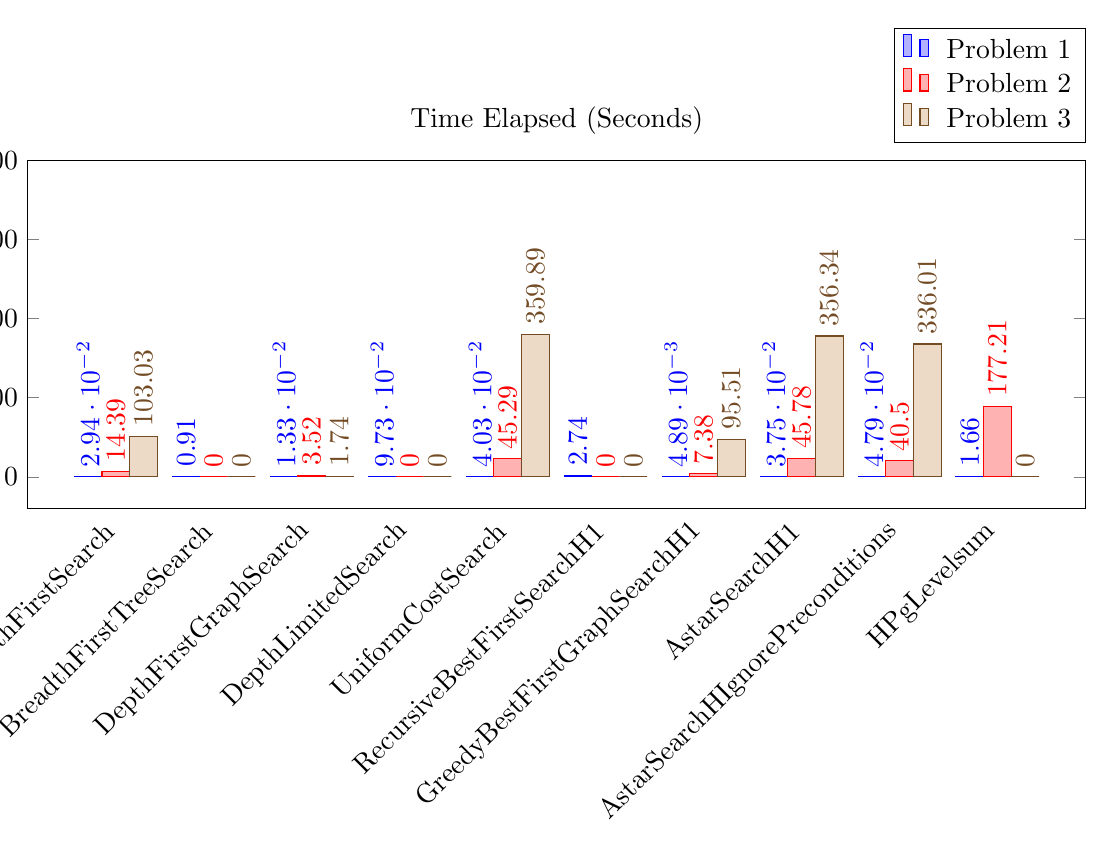
\begin{tikzpicture}[trim axis left, trim axis right]
	\begin{axis}[
			title={Time Elapsed (Seconds)},
			major x tick style = transparent,
			ybar=0pt,
			ymax=800,
			symbolic x coords={
				BreadthFirstSearch,
				BreadthFirstTreeSearch,
				DepthFirstGraphSearch,
				DepthLimitedSearch,
				UniformCostSearch,
				RecursiveBestFirstSearchH1,
				GreedyBestFirstGraphSearchH1,
				AstarSearchH1,
				AstarSearchHIgnorePreconditions,
				HPgLevelsum
			},
			height=6cm,
			x post scale=2.5,
			x tick label style={rotate=45,anchor=east},
			bar width=10pt,
			nodes near coords,
			every node near coord/.append style={rotate=90, anchor=west},
      legend cell align=left,
      legend style={
        at={(1,1.05)},
        anchor=south east,
        column sep=1ex
      }
			]

		\addplot table {
			X Y
			BreadthFirstSearch 0.029392972006462514
			BreadthFirstTreeSearch 0.910086860996671
			DepthFirstGraphSearch 0.01332990700029768
			DepthLimitedSearch 0.0973146399774123
			UniformCostSearch 0.040256563981529325
			RecursiveBestFirstSearchH1 2.7363686690223403
			GreedyBestFirstGraphSearchH1 0.004887217015493661
			AstarSearchH1 0.037505268992390484
			AstarSearchHIgnorePreconditions 0.04793940999661572
			HPgLevelsum 1.664410956989741
		};
		\addplot table {
			X Y
			BreadthFirstSearch 14.388099233008688
			DepthFirstGraphSearch 3.5191853329888545
			UniformCostSearch 45.29418297301163
			GreedyBestFirstGraphSearchH1 7.381141820020275
			AstarSearchH1 45.78383195499191
			AstarSearchHIgnorePreconditions 40.50242119200993
			HPgLevelsum 177.206022828992
			BreadthFirstTreeSearch 0
			DepthLimitedSearch 0
			RecursiveBestFirstSearchH1 0
		};
		\addplot table {
			X Y
			BreadthFirstSearch 103.0314349620021
			DepthFirstGraphSearch 1.7440492039895616
			UniformCostSearch 359.8916142139933
			GreedyBestFirstGraphSearchH1 95.50744679800118
			AstarSearchH1 356.3388120960153
			AstarSearchHIgnorePreconditions 336.01290577300824
			BreadthFirstTreeSearch 0
			DepthLimitedSearch 0
			RecursiveBestFirstSearchH1 0
			HPgLevelsum 0
		};
		\addlegendentry{Problem 1}
		\addlegendentry{Problem 2}
		\addlegendentry{Problem 3}
	\end{axis}
\end{tikzpicture}

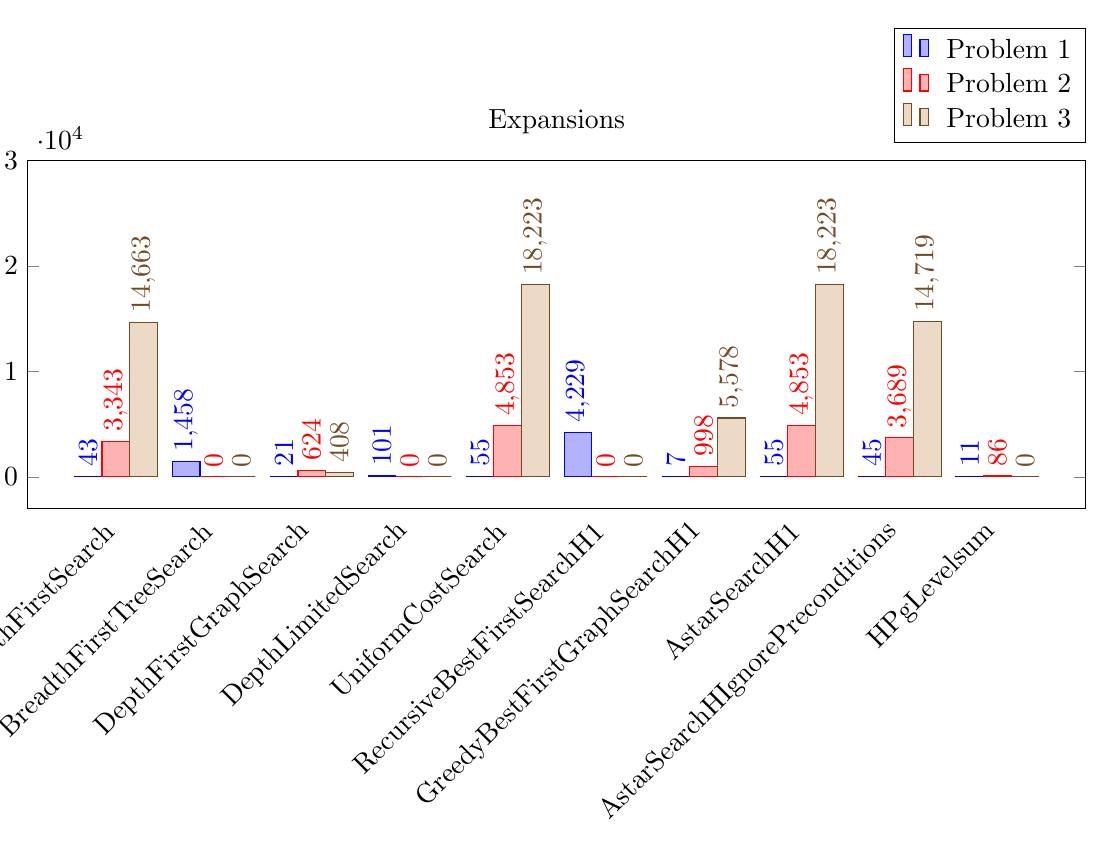
\begin{tikzpicture}[trim axis left, trim axis right]
	\begin{axis}[
			title={Expansions},
			major x tick style = transparent,
			ybar=0pt,
			ymax=30000,
			symbolic x coords={
				BreadthFirstSearch,
				BreadthFirstTreeSearch,
				DepthFirstGraphSearch,
				DepthLimitedSearch,
				UniformCostSearch,
				RecursiveBestFirstSearchH1,
				GreedyBestFirstGraphSearchH1,
				AstarSearchH1,
				AstarSearchHIgnorePreconditions,
				HPgLevelsum
			},
			height=6cm,
			x post scale=2.5,
			x tick label style={rotate=45,anchor=east},
			bar width=10pt,
			nodes near coords,
			every node near coord/.append style={rotate=90, anchor=west},
      legend cell align=left,
      legend style={
        at={(1,1.05)},
        anchor=south east,
        column sep=1ex
      }
		]

		\addplot table {
		X Y
		BreadthFirstSearch 43
		BreadthFirstTreeSearch 1458
		DepthFirstGraphSearch 21
		DepthLimitedSearch 101
		UniformCostSearch 55
		RecursiveBestFirstSearchH1 4229
		GreedyBestFirstGraphSearchH1 7
		AstarSearchH1 55
		AstarSearchHIgnorePreconditions 45
		HPgLevelsum 11
		};

		\addplot table {
		X Y 
		BreadthFirstSearch 3343
		BreadthFirstTreeSearch 0
		DepthFirstGraphSearch 624
		DepthLimitedSearch 0
		UniformCostSearch 4853
		RecursiveBestFirstSearchH1 0
		GreedyBestFirstGraphSearchH1 998
		AstarSearchH1 4853
		AstarSearchHIgnorePreconditions 3689
		HPgLevelsum 86
		};

		\addplot table {
		X Y
		BreadthFirstSearch 14663
		BreadthFirstTreeSearch 0
		DepthFirstGraphSearch 408
		DepthLimitedSearch 0
		UniformCostSearch 18223
		RecursiveBestFirstSearchH1 0
		GreedyBestFirstGraphSearchH1 5578
		AstarSearchH1 18223
		AstarSearchHIgnorePreconditions 14719
		HPgLevelsum 0
		};

		\addlegendentry{Problem 1}
		\addlegendentry{Problem 2}
		\addlegendentry{Problem 3}
	\end{axis}
\end{tikzpicture}

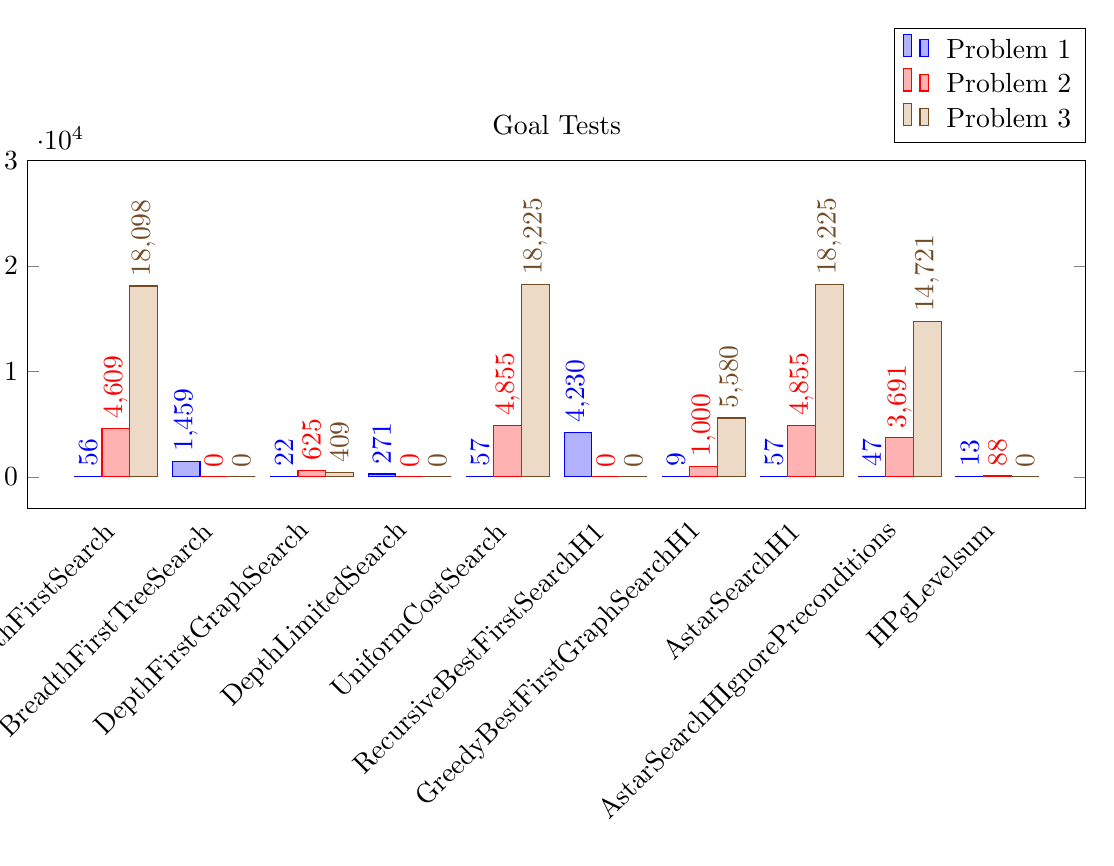
\begin{tikzpicture}[trim axis left, trim axis right]
	\begin{axis}[
			title={Goal Tests},
			major x tick style = transparent,
			ybar=0pt,
			ymax=30000,
			symbolic x coords={
				BreadthFirstSearch,
				BreadthFirstTreeSearch,
				DepthFirstGraphSearch,
				DepthLimitedSearch,
				UniformCostSearch,
				RecursiveBestFirstSearchH1,
				GreedyBestFirstGraphSearchH1,
				AstarSearchH1,
				AstarSearchHIgnorePreconditions,
				HPgLevelsum
			},
			height=6cm,
			x post scale=2.5,
			x tick label style={rotate=45,anchor=east},
			bar width=10pt,
			nodes near coords,
			every node near coord/.append style={rotate=90, anchor=west},
      legend cell align=left,
      legend style={
        at={(1,1.05)},
        anchor=south east,
        column sep=1ex
      }
			]

		\addplot table {
			X Y
			BreadthFirstSearch 56
			BreadthFirstTreeSearch 1459
			DepthFirstGraphSearch 22
			DepthLimitedSearch 271
			UniformCostSearch 57
			RecursiveBestFirstSearchH1 4230
			GreedyBestFirstGraphSearchH1 9
			AstarSearchH1 57
			AstarSearchHIgnorePreconditions 47
			HPgLevelsum 13
		};
		\addplot table {
			X Y
			BreadthFirstSearch 4609
			DepthFirstGraphSearch 625
			UniformCostSearch 4855
			GreedyBestFirstGraphSearchH1 1000
			AstarSearchH1 4855
			AstarSearchHIgnorePreconditions 3691
			HPgLevelsum 88
			BreadthFirstTreeSearch 0
			DepthLimitedSearch 0
			RecursiveBestFirstSearchH1 0
		};
		\addplot table {
			X Y
			BreadthFirstSearch 18098
			DepthFirstGraphSearch 409
			UniformCostSearch 18225
			GreedyBestFirstGraphSearchH1 5580
			AstarSearchH1 18225
			AstarSearchHIgnorePreconditions 14721
			BreadthFirstTreeSearch 0
			DepthLimitedSearch 0
			RecursiveBestFirstSearchH1 0
			HPgLevelsum 0
		};
		\addlegendentry{Problem 1}
		\addlegendentry{Problem 2}
		\addlegendentry{Problem 3}
	\end{axis}
\end{tikzpicture}

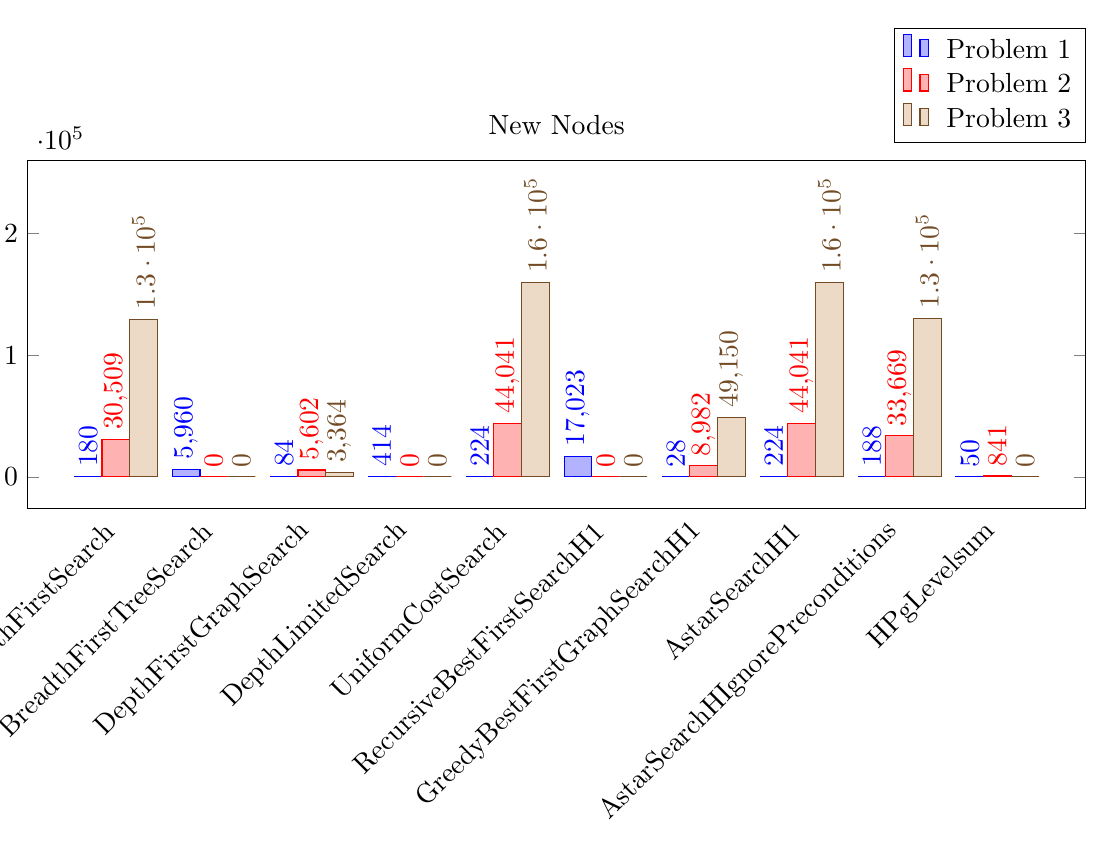
\begin{tikzpicture}[trim axis left, trim axis right]
	\begin{axis}[
			title={New Nodes},
			major x tick style = transparent,
			ybar=0pt,
			ymax=260000,
			symbolic x coords={
				BreadthFirstSearch,
				BreadthFirstTreeSearch,
				DepthFirstGraphSearch,
				DepthLimitedSearch,
				UniformCostSearch,
				RecursiveBestFirstSearchH1,
				GreedyBestFirstGraphSearchH1,
				AstarSearchH1,
				AstarSearchHIgnorePreconditions,
				HPgLevelsum
			},
			height=6cm,
			x post scale=2.5,
			x tick label style={rotate=45,anchor=east},
			bar width=10pt,
			nodes near coords,
			every node near coord/.append style={rotate=90, anchor=west},
      legend cell align=left,
      legend style={
        at={(1,1.05)},
        anchor=south east,
        column sep=1ex
      }
			]

		\addplot table {
			X Y
			BreadthFirstSearch 180
			BreadthFirstTreeSearch 5960
			DepthFirstGraphSearch 84
			DepthLimitedSearch 414
			UniformCostSearch 224
			RecursiveBestFirstSearchH1 17023
			GreedyBestFirstGraphSearchH1 28
			AstarSearchH1 224
			AstarSearchHIgnorePreconditions 188
			HPgLevelsum 50
		};
		\addplot table {
			X Y
			BreadthFirstSearch 30509
			DepthFirstGraphSearch 5602
			UniformCostSearch 44041
			GreedyBestFirstGraphSearchH1 8982
			AstarSearchH1 44041
			AstarSearchHIgnorePreconditions 33669
			HPgLevelsum 841
			BreadthFirstTreeSearch 0
			DepthLimitedSearch 0
			RecursiveBestFirstSearchH1 0
		};
		\addplot table {
			X Y
			BreadthFirstSearch 129631
			DepthFirstGraphSearch 3364
			UniformCostSearch 159618
			GreedyBestFirstGraphSearchH1 49150
			AstarSearchH1 159618
			AstarSearchHIgnorePreconditions 130437
			BreadthFirstTreeSearch 0
			DepthLimitedSearch 0
			RecursiveBestFirstSearchH1 0
			HPgLevelsum 0
		};
		\addlegendentry{Problem 1}
		\addlegendentry{Problem 2}
		\addlegendentry{Problem 3}
	\end{axis}
\end{tikzpicture}

\end{document}
